\chapter{Methods} % Main chapter title

\label{chap:methods} % For referencing the chapter elsewhere, use \ref{Chapter1} 

%----------------------------------------------------------------------------------------
[Pipeline Introduction]

To address of problem of localizing cortical areas processing semantic similarity and/or association, we use voxel-wise fMRI encoding to estimate local superiority of semantic representations. The human subjects' brain activity are recorded when they attentively listen to naturally spoken narrative stories from \cite{saint-exuperyPetitPrince1943}. We reconstruct features (regressors) using non-semantic signals\footnote{including acoustic energy, word presence and content word presence.} and semantic representation models tuned for semantic similarity and association. The model estimation are constructed using several sessions of fMRI recording, and the built model is validated by using data from the residual sessions.

\section{fMRI Acquisition and Preprocessing}

The fMRI experiment is designed and carried out by \cite{todorovicAnalysesIRMfLors2018}. 20 French native speakers (11 females, average age of 24.5 years-old, range 18-39 years-old, right handed according Edinburgh's inventory [TODO ref], without antecedent neurological or psychiatric disorders) are recruited among Neurospin [TODO details]'s volunteer inventory. The participants listened to the French audio book \parencite{saint-exuperyLittlePrinceFrench2011} divided into 9 blocks and were tested with comprehension multi-choice questions at the end of each block. During the listening period, a Siemens scanner scans the whole brain at 3 Tesla with multi-echo EPI sequence at 2 second-per-image rate. Each scanning session lasts at maximum 90 minutes. Each subject passes two sessions during the same day. 

The multi-echo procedure has a higher signal-to-noise ratio over mono-echo, thus it shows better activities in cortical areas [TODO read Kundu paper]. The voxel size, as a compromise, is fixed at a larger volume than classic modern fMRI recordings of  \(3.159 \times 3.159 \times 3.159 mm ^ 3\).

Please refer to appendix \ref{appsec:fmriacquisition} for a more detailed introduction, and to the original report (in French) \parencite{todorovicAnalysesIRMfLors2018} for comprehension question designs, fMRI session procedures and behavioral results.

The acquired MRI (anatomical and functional) data are then preprocessed with ME-ICA pipeline\footnote{Library available at \url{https://github.com/ME-ICA/me-ica}, commit \code{6ae63c7}.} \parencite{kunduDifferentiatingBOLDNonBOLD2012} to transform spatial normalization to MNI template and extract whole-brain BOLD signals. 

\section{Semantic Feature Embedding Construction}

To build numerical regressors for voxel models, we first obtain numerical representation of the semantic principles in question. We then validate their performance in similarity and association proximity evaluation ranking tasks before passing them to build fMRI regressors.

Since we do not have widely-used French semantic task benchmarks in disposition, our implementation of semantic embedding construction algorithms are tuned and validated on English data, then applied on French data. 


\subsection{Semantic Similarity Embedding}
\label{subsec:semanticsimilaritymethod}
To build semantic similarity representation, we use English WordNet \parencite{millerWordNetLexicalDatabase1995, millerWordNetElectronicLexical1998}, French WOLF \parencite{sagotBuildingFreeFrench2008} as our data source. For semantic entities encoded in an ontological graph, \cite{saediWordNetEmbeddings2018} propose an evaluation of semantic affinity by counting all the paths connecting two nodes representing entities. The paths are weighted by their length: shorter is the path, stronger is the semantic affinity. Equation \ref{eqn:randomwalk} illustrates the exact numerical calculation by taking \(M\) as the weighted adjacency matrix representation of the initial graph. 
\begin{equation}
    M_G^{(n)} = I + \alpha M + \alpha^2 M^2 + \dots + \alpha^n M^n \\
    M_G = \sum_{e=0}^{\infty}{(\alpha M)}^e = (I - \alpha M)^{-1}
\label{eqn:randomwalk}
    \end{equation}
 After computing the graph distance of between all pairs, a normalized Positive Point-wise Mutual Information transformation is applied to the matrix to reduce noises introduced by unbalanced word occurrence frequency. Finally a PCA is performed to reduce the dimensionality of the large matrix. 

We replicated Saedi et al.'s experiment using the reported optimal parameters\footnote{including graph random-walk decay factor, semantic relation weight attribution}. Our tests differed from the original work on semantic relation selection, vocabulary size and final dimensionality choice. 

As mentioned in the section \ref{subsection:hypsemantichub}, similarity-related relationships include synonymy, hypernymy, hyponymy, (adjectives as a) participle of verbs, (adjectives being) similar to and (adverbs) derived from adjectives. We test different set of combinations of relations to further confirm this argument (see section \ref{appsubsec:wnembeddingtests}).

As large matrix calculation is very memory-consumptive, in function of the available memory on the laboratory server\footnote{The computer is equipped with an octa-core Intel Xeon processors @ \code{3.70 GHz}, \code{32 GB} RAM, running Ubuntu \code{18.10}, Python \code{3.6.7} Anaconda.}, we selected the 15 000 most frequent words in WordNet and 20 000 in WOLF for fast in-memory computing, and then took 60 000 in WordNet and all words in WOLF (56665) for the optimal model performance. 

To determine the number of first principle components (PC) of the graph encoding word-wise proximity, we initially keep 8 000 PCs as potential candidate (see figure \ref{fig:SimDimensionSeletionVarRatio}). We apply a Savitzky-Golay filter of window size 100 and of first order on the difference of explained variance ratio (EVR), and visually select the cutting position around the first local minima with a following sufficiently wide valley (figure \ref{fig:SimDimensionSelectionVarRatioDiff}).

\begin{figure}
    \centering
    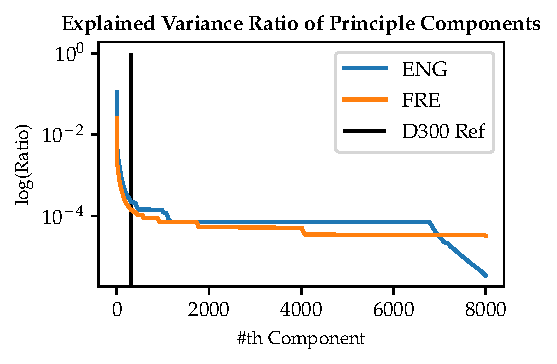
\includegraphics[scale=1]{Figures/SimDimensionSelectionVarRatio.pdf}
    \caption[Explained Variance Ratio of WordNet Embedding Principle Components]{The \code{log} of EVR of each PC in WordNet embedding space (\code{ENG}) and in WOLF embedding space (\code{FRE}). The PCs are ordered by their corresponding eigenvalues. The black vertical line is placed at the classic choice dimensionality of 300 as a reference.}
    \label{fig:SimDimensionSeletionVarRatio}
\end{figure}

\begin{figure}
    \centering
    \makebox[\linewidth]{
    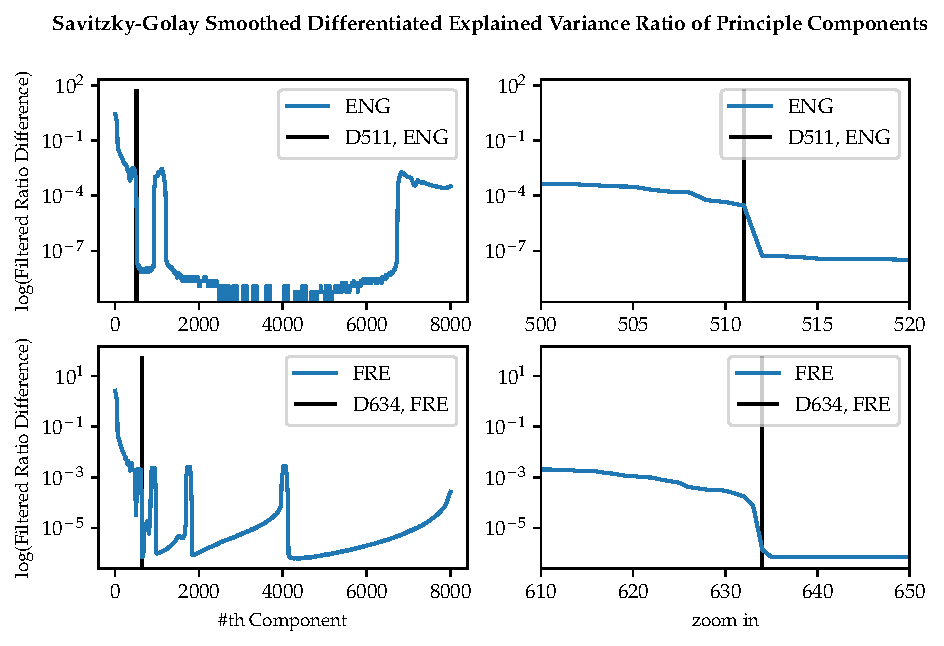
\includegraphics[scale=1]{Figures/SimDimensionSelectionVarRatioDiff.pdf}
    }
    \caption[Smoothed Differentiated EVR of WordNet Embedding PCs]{\textbf{Left panels}: The base signal is obtained by subtracting the neighbour components' EVR. \code{D511} in \code{ENG} and \code{D634} in \code{FRE} are visually selected on the left border of a sufficiently wide signal valley. }
    \label{fig:SimDimensionSelectionVarRatioDiff}
\end{figure}

% code Decorrelation_French.ipynb

\subsection{Semantic Association Embedding}

Under the assumption of the linear mixture of paradigmatic and syntagmatic information in classical statistical embeddings (refer to section \ref{subsection:hyplinearsemantics}), we extract association representations from classic statistical embeddings with equation \ref{eqn:linearmixture}, where \(M\) is the mixed semantic representation space, \(S\) being the similarity based space, \(P\) a learned projection matrix projecting the similarity space onto the mixed space, and the residual \(A\) being the association space. The embedding spaces of interest are \(S\) and \(A\), henceforth respectively noted as \emph{SIM}(short for \textbf{sim}ilarity) and \emph{ASN} (\textbf{as}sociatio\textbf{n}). The two auxiliary spaces are \(P\) and \(M\), noted as \emph{SIG} (\textbf{si}milarity projected on Dep\textbf{G}love) and \emph{MIX} (\textbf{mix}ed).

Each row of the three semantic space matrices represents a lexicon. Since different semantic spaces have different vocabulary setting, we keep the intersection of two vocabularies of one same language in later stages. The lexicon alignment between the English spaces is based on the lexicon orthography, which is computed automatically. We hand coded rules to tidy up WOLF vocabulary and transformed DepGloVe's complex POS tag entries into WOLF's relatively simple set. Then French vocabulary is aligned with the additional POS information. Finally we manually check the vocabulary coverage of validation dataset and fMRI stimuli words and corrected relevant algorithm erroneous results. [TODO, code reference for manual correction set] % code Decorrelaation_French.ipynb & Text Preprocessing.ipynb

The projection weight is learned via a general linear model (GLM) [TODO ref python], with the computational objective to minimize the L-2 norm of \(A\).

\begin{equation}
M = S.P + A
\label{eqn:linearmixture}
\end{equation}

As baseline models, for English we use GloVe \parencite{penningtonGloveGlobalVectors2014} trained on Common Crawl with 840B tokens, 2.2M cased vocabulary and 300-dimension vectors \footnote{Available at \url{https://nlp.stanford.edu/projects/glove/}}. For French we use DepGloVe \parencite{delaclergerieDepGloveSmallServer}. 

English GloVe embeddings provide vectorial representations for lexicons. However since French nouns, verbs and adjectives have various inflective forms, this inflection can thin out captured semantic information if each specific form does not have sufficient frequency in a given corpus. DepGloVe aggregates the semantic information by lemmatizing the tokens and attribute them with a part-of-speech tag. Our textual data including validation task benchmarks and fMRI stimuli are transformed to align with this strategy. 

\subsection{Embedding Validation}

Since many assumptions are made for the structure and content of semantic representation spaces, the preliminary tests serve as an behavioral assurance. 

The semantic ranking task depends on a database of word-pairs, each attributed with a proximity score (usually annotated by human) which measures the proximity in terms of the semantic property defined by the task. Each computational semantic representations space are provided with a proximity measure, which could be based on graph distances or vectorial distances. The score of semantic ranking task is computed by calculating pearson's and spearman's correlation coefficient \code{r} between the model based word-pair proximity and the baseline. 

Conformably with other works on semantic model evaluation [TODO Refs] \parencite{saediWordNetEmbeddings2018}, we use benchmark data provided by \cite{rubensteinContextualCorrelatesSynonymy1965} (\textbf{RG1965}), \cite{agirreStudySimilarityRelatedness2009} (\textbf{WS353-Similarity}) and \cite{hillSimLex999EvaluatingSemantic2015} (\textbf{SimLex-999}) to evaluate English semantic similarity models. The only available benchmark conceived for evaluating association relations is \textbf{WS353-Association}.

\label{subsection:frenchbenchmarkdataconstruction}
\cite{freitasSemanticRelatednessAll2016} provides translation for those benchmarks in French, however the provided proximity scores are heterogeneous with the original rankings. Scores for French \textbf{SimLex-99} are given by a computer semantic model, while \textbf{WS353} scores are identical with English data. The latter configuration is problematic since in different languages the translation are not exact mappings between words, and the proximity are subject to the word choice. We manually corrected the erroneous translation of word pairs and eliminated or replaced word-pairs that are translated to the same word. Scores for the replaced word-pairs are retrieved from the English dataset. Additionally, we also added POS tags for the continuity with the tested embedding spaces. The built French benchmark data suffer from the lack of real human judgement data, thus they serve merely as indicators of semantic model performance. The modified benchmarks are made available on GitHub\footnote{commit \code{c97583f}, \url{https://github.com/nicolasying/Similarity-Association-Benchmarks}}.

\section{fMRI Voxel-Wise Encoding}

In this project and many other similar works [TODO, refs], we consider the BOLD signal as a temporal signal linearly additively composed by variously independent functional components, which themselves are convolutions of separate neuron activations with a hemodynamic function: 

\begin{equation}
    \text{BOLD}_{\text{theory}, j}(t) = \sum_i {\alpha_{i,j} * f_{i}(t) * \text{hrf}(t)}
\label{eqn:boldlinear}
\end{equation}

, where \(\alpha_{i,j}\) is the linear coefficient of the \code{i}-th component in the voxel \code{j}, \(f_{i}\) is a function modeling the \code{i}-th independent functional activation, and \(\textnormal{hrf}\) is the hemodynamic function (we use the model used in SPM at oversampling rate of 10 [TODO ref, nistat, SPM]). [TODO, insert figure of hrf sample] 

Since different voxels contain neurons of distinct (yet possibly similar) activation profile towards stimuli, the coefficient associated with each functional component are also different for each voxel. For example, in setting of an auditive comprehension task, we can have voxels which are not implicated having all the \(\alpha_{i}\) in equation \ref{eqn:boldlinear} systematically set to 0, and voxels containing neurons primarily associated with low-level auditive functions having non-zero \(\alpha\)s for low-level auditive features.

\subsection{fMRI Textual Stimuli Preparation} 

% notebook, Text Preprocessing.ipynb
For the generation of regression features for fMRI encoding, we perform a lemmatization of the Little Prince story. First the text is parsed with syntax dependence analysis with \code{spaCy}\footnote{version \code{2.0.16}} library and each token is attributed with a POS tag. We then used \code{FrenchLefffLemmatizer}\footnote{commit \code{ba1ef2b}. The library is publicly available on GitHub, \url{https://github.com/ClaudeCoulombe/FrenchLefffLemmatizer.}}\parencite{sagotLefffFreelyAvailable2010} library to return verbs to the infinitive form and other words to masculine singular form. POS info from \code{spaCy} helps to resolve lemmatisation ambiguity. The pipeline-generated lemma and POS tags are then manually verified.

\subsection{Regression Feature Generation}
\label{subsec:regressionfeaturegeneration}
The exact transcription of the audiobook is performed by \cite{todorovicAnalysesIRMfLors2018}. With jtrans and Praat, the authors aligned the audio with the text by marking the onset and offset of each pronounced word in the story. To pin down the BOLD signal at a given time, we reconstruct temporal regressor functions by firstly build \(f_{i}\) in equation \ref{eqn:boldlinear}, which is essentially a sequence of bumps each occurs at the onset of a word (or content word), then we concatenate the convoluted \(D\) sequences into a design matrix of \(D\) columns.

% code TextFineTuning\LPP Onset\Lemmatisation Feature Gen.ipynb, generate_regressors.py, events2reg.py
We used four classes of regressors to reconstruct human listening comprehension processing cerebral activities:
\begin{enumerate}
	\item \code{RMS} (Acoustic Energy), which is the root means square of audio wave amplitude calculated on a sliding window of 10 msec, with Octave\footnote{\url{https://www.gnu.org/software/octave}}.
	\item \code{WRATE} (Word Presence), a binary temporal sequence indicating if a word is being pronounced at a given time.
	\item \code{CWRATE} (Content Word Presence), a similar binary feature to \code{WRATE}, which indicates the presence of a content word, determined by the POS tag (noun, verb, adverb and adjective) of the lemmatised text.
	\item \code{SIM/ASN/SIG/MIX} (Semantic Embedding-Based Features), a multi-dimensional feature set, which takes the value of the semantic vector of the current content word from a certain representation model defined in \(\mathbb{R}\) space. [TODO rephrase]
\end{enumerate}
The four classes include informative dimensions (\code{RMS} and \code{WRATE}) reported by post-hoc analysis of \cite{todorovicAnalysesIRMfLors2018}. 

For the ease of later feature selection, we systematically performed orthonormalization of the convoluted feature sequences to cancel the co-linearity of the regressors. This is implemented with Gram-Schmidt process, where the orthogonal sequence is defined by the precedent order of regressor classes, and the semantic embedding based regressors inner-class order is either given by the semantic model (e.g. \code{ASN/SIG/MIX}) or by PCA (e.g. \code{SIM}). 


\subsection{Feature Selection for Specific Corpus}
% notebook, Embedding Dimension Selection for LPP.ipynb

As \cite{saint-exuperyPetitPrince1943} cannot cover all the vocabulary of the four semantic embeddings, we suspect that there might be some semantic dimensions in the semantic spaces that are not fully exhibited in this project. It is in our interest to simplify the design matrix to avoid overfitting and accelerate model fitting computation. Therefore we take an investigation of the 9 design matrices (one per fMRI block) by computing each design matrix's variance of individual regressors. After orthonormalization, the variance of regressors in higher dimension positions are of a much smaller order than the first regressors especially for PCA-factored semantic spaces. By applying a threshold on regressor variance we can filter out uninformative ones. The value of threshold is determined visually to limit the number of informative regressors under 200.

\subsection{Ridge Regression with Step-Forward Feature Selection, Grid Search and Cross Validation}
% Ridge regression with stepwise feature selection, GridSearch Alpha 
% Github code
The fMRI encoding protocol is to find a function projecting our theoretical feature regressors onto BOLD amplitudes. We assume that the target BOLD value is linearly composited by individual regressors, similar in equation \ref{eqn:boldlinear}. The coefficients in the equation above is determined by the minimization of the difference between the predicted value given by the equation and the real value, on a set of discrete timestamps. This is a typical regression problem tackled in Machine Learning. The computation of the coefficients is named \emph{training} or \emph{fitting} of the model. The performance of a fitted model trained on a dataset is evaluated on the accuracy of its predictions on unseen data, which indicates its \emph{generalized predictive power}.

In each fMRI session block we have around 300 whole-brain images (refer to section \ref{appsubsec:fmridata} for more details), totaling 2937 observations. Researchers \parencite{huaOptimalNumberFeatures2005} found that in GLM the optimal number of uncorrelated informative features is \(N - 1\) where \(N\) is the number of observation, and \(\sqrt{(N)}\) if features are correlated. Although we have numerically de-correlated the regressors, we nevertheless cannot assume the conceptual dependency. Thus 200 regressors might outnumber the recommended feature size. To avoid potential overfitting of regression models, we use Ridge regression [TODO ref, equation] to penalize the attribution of large coefficients to reduce potential noises, therefore promote generalizability of a fitted model.

Ridge regression fitting algorithm requires a hyper-parameter (\(\alpha\)) to adjust the severity of large-coefficient penalty. There's no empirically predetermined optimal choice of the value, thus we test a range of candidates by fitting different models and evaluate their performance. 

We also assumed the heterogeneity of voxel activation profile towards different functional features. In order to maximize the predictive power of models, we explicitly filter out some particular features on some model candidates. Limited by the computation time, we do not test all the combination of individual features which could results in an exponential complexity, but use \emph{step-forward} feature selection by the order of feature classes (section \ref{subsec:regressionfeaturegeneration}).

For each voxel of a subject and each combination of feature selection and \(\alpha\) value candidate\footnote{Please refer to section \ref{appsubsec:regressionparameters} for tested \(\alpha\) value, feature selections.}, we adopt the common practice of Cross Validation (CV), where we generate 9 different regression models by training on 8 runs of fMRI recording, and test their performance on the left run by computing the coefficient of determination (\code{r2}) and Pearson's \code{r} by comparing model predicted BOLD values and real observations. \code{r2} measures the proportion of the variance in the BOLD signal that is predictable from the feature regressor data. An \code{r2} of 1 indicates that the regression predictions perfectly fit the data. Pearson's \code{r} measures the linearity between the predicted BOLD signals and the real values. A \code{r} of 1 indicates a perfect prediction too, and near-0 or negative values indicate a bad fit. Positive \code{r2} can be computed from \code{r}, according to the definition of \code{r2} used in \code{scikit-learn}.

We normalized all feature regressors and voxel-wise fMRI signal sequences for the facility of inter-individual comparison and group-level analysis. To reduce the total computation time, we filtered out unimportant voxels in the images by computing a multi-EPI mask.\footnote{The \code{nilearn.masking.compute\_multi\_epi\_mask} uses the mask-finding algorithms to extract masks for each session of subject, and then keeps only the main connected component of a given fraction  of the intersection of all the masks.}

\section{Analysis}

The Ridge regression pipeline results to \[ \lvert \text{Subject} \rvert \times \lvert \text{Voxels} \rvert \times \lvert \alpha \text{candidates} \rvert \times \lvert \text{feature selection} \rvert \times \lvert \text{CV} \rvert \] for each semantic space. 


\subsection{Incremental Nested Model Sequence}

First we investigate the validity of regression results. For each individual, we averaged the \code{r2} score of 9 CVs, then selects the highest \code{r2} among \(\alpha\)s and feature selections within feature classes. As regression models may overfit, the addition of extra feature does not necessarily translate into a higher performance.

Before roaming in undiscovered land of semantic embeddings, by plotting the whole-brain map of \code{r2}, we expect to recover at least auditive cortical areas for \code{RMS} feature regression. At confirmation of validity of basic results, we additionally visualize the improved regression results by integrating higher level features and the improvement contrast. 

The statistical significance of improvement is computed by Wald F-test. The Wald F-test compares the residual sum of squares (\code{RSS}) of a restricted model and a full model containing the former one, with the null hypothesis suggesting that the full model does not provide a significantly better data fit than the restricted one. The Wald test penalizes large feature set, and takes the number of observations into account. The \code{RSS} is computed from \code{r2} given that the data are centered and normalized. [TODO deduction]

At individual analysis level, for each contrast of each individual voxel, we compute \( \lvert \alpha \text{ candidates} \rvert \times \lvert CV \rvert \) F-tests and we select the most significant raw p-value. We then plotted the statistical map by thresholding the p-value by uncorrected 0.05, uncorrected 0.001 and multi-comparison corrected 0.05. For group analysis, [TODO?]

\subsection{Embedding Contrasts}
[TODO, Design matrix comparison]
The key comparison of regression results is the contrast between \code{SIM} and \code{ASN} semantic models. The comparison is inspired by the non-nested model comparison pipeline \parencite{merkleTestingNonnestedStructural2016}. Our method is divided into two steps: first we verify the structural difference between the design matrices given by each model, second we compare the model's regression results if the design matrices are found nonequivalent. The pipeline is detailed in section \ref{appsubsec:nonnestedcompmeth}.

We conceived two statistical tests on regression result metrics, in hope of finding converging evidences. Each test produces a voxel-level whole-brain statistical map.

\subsubsection{Paired t-test on Pearson's \code{r}}

With Fisher's transformation, we can bring Pearson's \code{r} to a normal distribution. [TODO, results visualize histogram] We select the best \code{Z}-score resulted from the transformation among \( \lvert \alpha \text{ candidates} \rvert \times \lvert \text{feature selection}  \rvert \), resulting to \( \lvert \text{Subject} \rvert \times \lvert \text{CV} \rvert \) observations of semantic model contrast. Individual contrasts are computed on \(\lvert \text{CV} \rvert \) observations, and group analysis is based on all data points.

\subsubsection{Wilcoxon Signed-Rank Test on \code{r2}}

The \code{r2}s follow distributions described by \(F(k-1, n-k)\), where \(k\) is the number of features and \(n\) is the number of observation. Since across semantic models, the feature dimensions are heterogeneous, \code{r2} scores have distinct score distributions. Therefore we adopted the nonparametric Wilcoxon Signed-Rank test to test the significance of \code{r2}-differences between semantic models. 

For individual contrasts, since \(\lvert \text{CV} \rvert < 20\), the Wilcoxon test falls back to a t-test.

\subsection{ROI-level Analysis}

With Region-of-Interest (ROI) analysis, we aim to filter out inter-subject variances and find relatively stable loci of each semantic network. From the relevant literatures reporting the activation peaks of semantic tasks [TODO, refs], we replicated \cite{pattersonWhereYouKnow2007}'s peak selection method to select the reported peaks,
% code ROI\Tal2MNI_ROI_gen.ipynb
and obtained the list of ROI by constructing a 7-mm diameter sphere around the peak. [TODO, figure of ROIs]

We completed the ROI list by intersecting the original ROI mask with gray-matter mask, and added classic brain anatomical areas. [TODO list of ROI]

\subsubsection{ROI Statistical Test}
We computed the ROI-average \code{r} and \code{r2}, and used the same tests as voxel-wise analysis. 

Additionally, we also experiment with ROI-wise Wald-test. We first compute ROI F-score and p-value, then threshold p-value by different degrees of significance. The model contrast is computed by subtracting the number of significant observations of each model.